%%%%%%%%%%%%%%%%%%%%%%%%%%%%%%%%%%%%%%%%%%%%%%%%%%%%%%%%%%%%%%%%%%%%%%%%%%%%%%%%
%2345678901234567890123456789012345678901234567890123456789012345678901234567890
%        1         2         3         4         5         6         7         8

\documentclass[spanish, letterpaper, 12 pt, conference]{ieeeconf}  % Comment this line out
% if you need a4paper
%\documentclass[a4paper, 10pt, conference]{ieeeconf}      % Use this line for a4
% paper

\IEEEoverridecommandlockouts                              % This command is only
                                                          % needed if you want to
                                                          % use the \thanks command
\overrideIEEEmargins
% See the \addtolength command later in the file to balance the column lengths
% on the last page of the document

\usepackage[utf8]{inputenc}
\usepackage[T1]{fontenc}
\usepackage[spanish]{babel}
\usepackage{hyperref}
\usepackage{float}
\usepackage{graphicx}
\usepackage[spanish]{babel}
\renewcommand\spanishtablename{Tabla}

% The following packages can be found on http:\\www.ctan.org
%\usepackage{graphics} % for pdf, bitmapped graphics files
%\usepackage{epsfig} % for postscript graphics files
%\usepackage{mathptmx} % assumes new font selection scheme installed
%\usepackage{mathptmx} % assumes new font selection scheme installed
%\usepackage{amsmath} % assumes amsmath package installed
%\usepackage{amssymb}  % assumes amsmath package installed

\title{\LARGE \bf
Crecimiento económico y su relación con energías limpias en la región latinoamericana
}

%\author{ \parbox{3 in}{\centering Huibert Kwakernaak*
%         \thanks{*Use the $\backslash$thanks command to put information here}\\
%         Faculty of Electrical Engineering, Mathematics and Computer Science\\
%         University of Twente\\
%         7500 AE Enschede, The Netherlands\\
%         {\tt\small h.kwakernaak@autsubmit.com}}
%         \hspace*{ 0.5 in}
%         \parbox{3 in}{ \centering Pradeep Misra**
%         \thanks{**The footnote marks may be inserted manually}\\
%        Department of Electrical Engineering \\
%         Wright State University\\
%         Dayton, OH 45435, USA\\
%         {\tt\small pmisra@cs.wright.edu}}
%}

\author{Geykel Hodgson, Aarón Sibaja }

% <-this % stops a space
%\thanks{*This work was not supported by any organization}% <-this % stops a space
%\thanks{$^{1}$H. Kwakernaak is with Faculty of Electrical Engineering, Mathematics and Computer Science,
%        University of Twente, 7500 AE Enschede, The Netherlands
%        {\tt\small h.kwakernaak at papercept.net}}%
%\thanks{$^{2}$P. Misra is with the Department of Electrical Engineering, Wright State University,
%        Dayton, OH 45435, USA
%        {\tt\small p.misra at ieee.org}}%



\begin{document}



\maketitle
\thispagestyle{empty}
\pagestyle{empty}


%%%%%%%%%%%%%%%%%%%%%%%%%%%%%%%%%%%%%%%%%%%%%%%%%%%%%%%%%%%%%%%%%%%%%%%%%%%%%%%%
\begin{abstract}

This electronic document is a "live'' template. The various components of your paper [title, text, heads, etc.] are already defined on the style sheet, as illustrated by the portions given in this document.

\end{abstract}


%%%%%%%%%%%%%%%%%%%%%%%%%%%%%%%%%%%%%%%%%%%%%%%%%%%%%%%%%%%%%%%%%%%%%%%%%%%%%%%%
\section{Introducción}

El acceso a la electricidad es un pilar fundamental para el bienestar humano, el desarrollo económico y la disminución de la pobreza. Asegurar que todos los habitantes tengan acceso a la energía corresponde a un desafío constante para cualquier nación.

Lamentablemente la mayor parte de los sistemas de energía tienen importantes impactos ambientales. Los sistemas eléctricos están dominados por hidrocarburos  como el carbón, petróleo y gas los cuales producen $CO_2$ y otros gases que recrudecen el efecto invernadero. 

Durante los últimos años se ha dado un cambio de mentalidad por parte de muchos países, apostando por acciones que reduzcan el impacto ambiental. Muchos de los esfuerzos de los países se centran en  cumplir demandadas que permitan propiciar un cambio positivo para el medio ambiente y así evitar un cambio catastrófico en la humanidad. El mundo necesita una transición significativa  de sus fuentes de energía.

Añadido a que muchos autores han afirmado que el acceso y producción de la electricidad se encuentran fuertemente relacionadas al incremento o disminución del PIB de un país, en este artículo se pretende elaborar una visualización que permita analizar el comportamiento de los países latinoamericanos durante el 2000 y 2015, utilizando índices que permitan comparar las fuentes de energías (renovables y no renovables) que consumen y producen  los países, haciendo hincapié en el uso de energías limpias y su relación con el PIB.


\section{Trabajo Previo}

La electricidad corresponde se encuentra fuertemente relacionada al progresoy éxito de una nación.Un cantidad significante de textos y artículos han demostrado cómo el crecimiento  de la actividad económica de un país se encuentra relacionado con el uso de la electricidad. Esto evidencia un crecimiento en la población y en la generación de bienes y servicios \cite{chen_relationship_2007}. 

El PIB  corresponde a la suma del sector  industrial, agricultura y de servicios de un país, en otras palabras, el valor en el mercado de sus productos y servicios. El sector agricultura y de servicios son sectores poco dependientes de la electricidad sin embargo el sector industrial si depende mayormente de la electricidad. Esto da cómo que la relación entre el PIB y el consumo de electricidad en países que basan mayormente su economía en el sector industrial. Para el 2017, 20$\%$ del PIB en Estados Unidos estaba conformada por el sector industrial \cite{noauthor_why_2014}. 

Algunos países que pertenecen al OCDE (Organización para la Cooperación y el Desarrollo Económicos ) cómo por ejemplo: Canadá, Reino Unido, Suiza, USA, Alemania y Colombia tienen economías fuertemente influenciadas por  la manufactura, sin embargo continuamente se actualizan a tecnologías que hacen uso de un menor recurso eléctrico y son más eficientes \cite{noauthor_link_nodate}. Los paises que no forman parte del OCDE cómo China, India y Brazil, presentan economías en crecimiento generalmente basadas en sector manufactura. Estas economías en particular presentan tecnologías más antiguas que requieren un mayor consumo de energía para poder generar bienes. En el 2011 el total de uso de energía de los países que no pertenecen al OCDE sobrepasó a los miembros del OCDE. Esto evidencia que probablemente la mayor cantidad de consumo eléctrico en el futuro va a concentrar en los paises que no forman parte del OCDE y el camino que elijan para sus respectivas economías. 



\section{Metodología}
Para la realización de este trabajo se decidió utilizar la metodología propuesta por Benjamín Fry \cite{fry2008visualizing}, este método consta de siete etapas:
\begin{itemize}
    \item \textbf{Recolectar datos: } 
    esta etapa consiste en buscar y obtener el conjunto de datos que vamos a utilizar, lo principal es conseguir fuentes de datos confiables, provenientes de otros estudios académicos o algún organismo oficial. En esta fase también se define como los datos recolectados van a ser accedidos por los usuarios.
    \item \textbf{Estructuración de los datos: } 
    una vez que se tienen datos confiables, hay que ordenarlos y categorizarlos para que estos adquieran una estructura bien definida. Si lo datos no están estructurados correctamente se dificulta el análisis y la visualización de los mismos.
    \item \textbf{Filtrar: }
    en este paso se debe decidir desde el punto de vista de la visualización cuales datos son útiles y aportan información relevante. Los datos que no se consideren relevantes son filtrados y no se toman en cuenta para la representación.
    \item \textbf{Extraer: }
    se procede a convertir, los datos relevantes, en variables que denoten los valores o cantidades que necesitamos analizar y mostrar a través de la visualización. Esto se logra al aplicar métodos estadísticos o de minería de datos que permitan colocar los datos en un contexto matemático.
    \item \textbf{Representar:}
    se escoge un modelo visual básico (Gráfico de barras, arboles, listas, entre otros), apropiado para una visualización clara y concisa de las variables creadas en el paso anterior.
    \item \textbf{Refinar: }
    trabajar de forma iterativa sobre el modelo visual básico con el fin de mejorarlo y que sea capaz de transmitir la información de forma clara, además debe ser atractivo y cautivador para el usuario.  
    \item \textbf{Interactuar: }
    agregar elementos que permitan al usuario la manipulación y el control de las características que son visibles. Los usuarios deben poder seleccionar diferentes rangos de datos e intervalos de tiempo que le permitan analizar la información presentada desde múltiples puntos de vista.  
\end{itemize}


\section{Procedimiento}

\subsection{Recolección de datos}

La búsqueda y recolección de datos se hizo con ayuda del buscador \href{https://www.google.com/publicdata}{Google Public Data Explorer}, que proporciona datos y pronósticos públicos de una variedad de organizaciones internacionales e instituciones académicas, incluidos el Banco Mundial, la OCDE, Eurostat y la Universidad de Denver. 
Como resultado de la búsqueda decidimos utilizar la base de datos del Banco Mundial, la cual proporciona acceso libre y gratuito a un conjunto completo de datos sobre el desarrollo en los países a través de todo el mundo. Los datos usados para la construcción de la visualización pueden ser consultados en el siguiente enlace: \url{https://datos.bancomundial.org/} 

\subsection{Estructuración  de  los  datos}

Para la estructuración, consulta y acceso a los datos se utilizo el servicio de \href{https://cloud.google.com/products/bigquery/}{BigQuery}.
BigQuery es un almacen de datos en la nube sin servidores, gratuito para consulta de bases de datos publicas y altamente escalable. Permite consultar grandes cantidades de datos estructurados o semi-estructurados mediante el uso de lenguaje SQL, lo que nos facilito la revisión y análisis de los datos.  
Otra de las ventajas a demás permite la integración y consulta muchas bases de datos publicas entre las cuales esta la base de datos del Banco Mundial.

\subsection{Filtrar}

La base de datos del Banco Mundial contiene mas de 1400 diferentes indicadores, cada uno de los cuales tienen un código único que los identifica. La selección de los indicadores relevantes, para la visualización, se hizo buscando de códigos de indicadores que estuvieran relacionados ya sea al PIB, combustibles o energía. De esta forma se logro reducir el numero de indicadores a solamente 48. Estos fueron luego estudiados uno a uno con mas detenimiento para comprobar cuales aportaban información relevante. Al final del proceso solo 12 se consideraron para ser incluidos en la visualización.

Los 12 indicadores seleccionados se listan en la tabla \ref{table_indicartors}.

\begin{table*}[h]
\caption{Códigos para los indicadores de producción, consumo, tipos de energía y crecimiento de PIB. Banco Mundial}
\label{table_indicartors}
\begin{center}
\begin{tabular}{|c||c|}
\hline
Código & Descripción \\
\hline
EG.USE.COMM.FO.ZS   &  Consumo de energía procedente de combustibles fósiles (\% del total)\\
\hline
EG.FEC.RNEW.ZS  &  Consumo de energía renovable (\% del total)\\
\hline
EG.ELC.FOSL.ZS  &  Producción de electricidad a partir de fuentes de petróleo, gas y carbón (\% del total)\\
\hline
EG.ELC.RNEW.ZS  &  Producción de energía eléctrica renovable (\% del total)\\
\hline
NY.GDP.MKTP.KD.ZG & Crecimiento del PIB per cápita (\% anual)\\
\hline
EG.ELC.COAL.ZS & Producción de electricidad a partir de carbón  (\% del total)\\
\hline
EG.ELC.NGAS.ZS & Producción de electricidad a partir de fuentes de gas natural (\% del total)\\
\hline
EG.ELC.PETR.ZS & Producción de electricidad a partir del petróleo (\% del total)\\
\hline
EG.ELC.HYRO.ZS & Producción de electricidad a partir de fuentes hidroeléctricas (\% del total)\\
\hline
EG.ELC.NUCL.ZS & Producción de electricidad a partir de fuentes nucleares (\% del total)\\
\hline
EG.ELC.RNWX.ZS & Producción de electricidad a partir de fuentes renovables, excluida la hidroeléctrica (\% del total)\\
\hline
\end{tabular}
\end{center}
\end{table*}


\subsection{Extraer}

En este caso no hizo falta aplicarle ningún tipo de conversión a los datos pues estos ya se encontraban en porcentajes lo que facilita la representación y corporación  de los mismos.

\subsection{Representar}

Para el diseño de la visualización optamos por usar otra de las herramientas que brinda la plataforma de Google, esta vez Data Studio cuya función principal es la creación de informes con visualización de datos. Una de las ventajas que provee la herramienta es la facilidad de integración con BigQuery servicio que usamos para estructurar, consultar y manipular en general los datos.

Otro de los aspectos que consideramos de Data Studio es que permite la inclusión, en los reportes, de gráficos personalizados desarrollados en JavaScript. Esto amplia considerablemente la capacidad de generar mejores y mas variadas visualizaciones, a su vez hace que la herramienta sea muy flexibilidad y adaptable ya que existen infinidad de recursos y librerías para la creación de gráficos y visualizaciones en JavaScript.        

En la figura \ref{fig:version_1} se pueden observar 3 tipos gráficos, seleccionados en la primera versión, para representar los diferentes indicadores.

El primer gráfico (figura \ref{fig:mapv1}) se representa el promedio del porcentaje anual del consumo de energía procedente de combustibles por país. Donde la escala de color indica un mayor o menor porcentaje de consumo; entre mas roja se la tonalidad implica que el país tiene un mayor consumo de energías procedentes de combustibles fósiles. Caso contrario entre mas verde la tonalidad implica un menor consumo. Por ultimo se trata de identificar con el color gris a los países con un consumo medio, es decir el consumo es menor al 60\%.

En siguiente gráfico visible en la figura \ref{fig:pibv1} representa el porcentaje de crecimiento del producto interno bruto (PIB) per capita a través del tiempo para cada país.

Y para finalizar representamos el porcentaje promedio de producción de energía por tipo de energía por país usando un gráfico de barras 100\% como se aprecia en la figura \ref{fig:tiposv1}.   

\begin{figure}[h]
\begin{subfigure}{\textwidth}
  \centering
  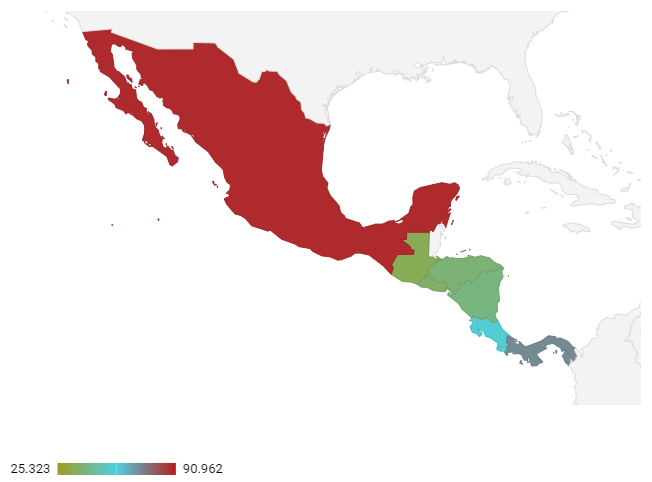
\includegraphics[width=.8\linewidth]{./img/mapav1.png}
  \caption{Geo-mapa con el porcentaje promedio anual del consumo de energías procedentes de hidrocarburos. }
  \label{fig:mapv1}
\end{subfigure}%
\begin{subfigure}{\textwidth}
  \centering
  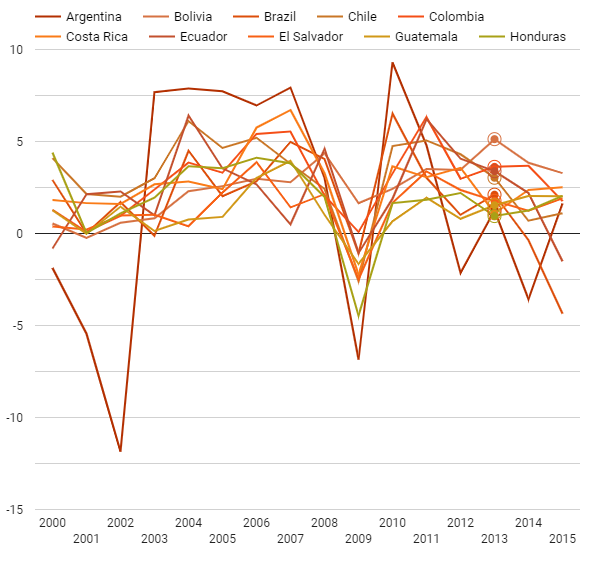
\includegraphics[width=.8\linewidth]{./img/PIBv1.png}
  \caption{Gráfico lineal del PIB anual por país.}
  \label{fig:pibv1}
\end{subfigure}
\begin{subfigure}{\textwidth}
  \centering
  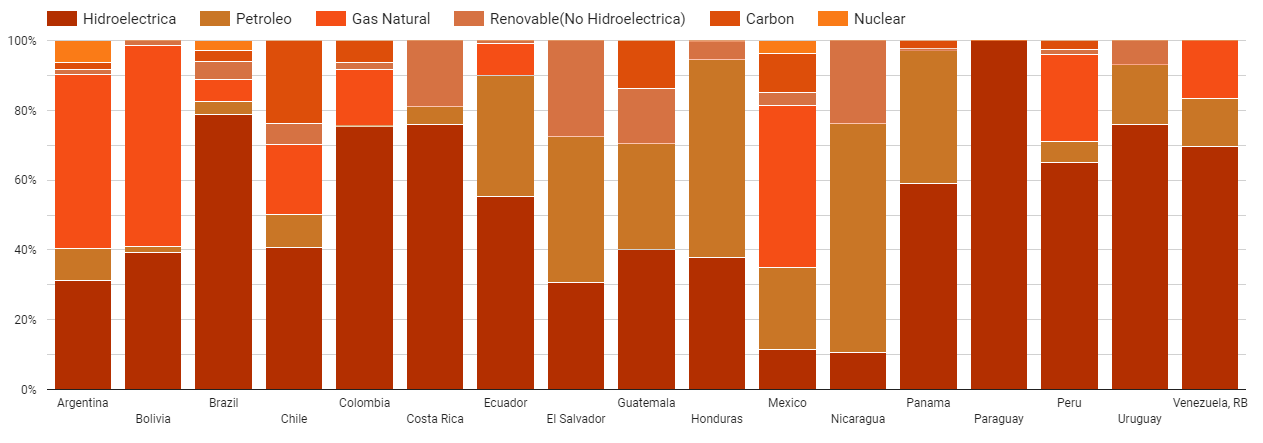
\includegraphics[width=.8\linewidth]{./img/tiposv1.png}
  \caption{Gráfico de barras 100\% con los tipos de energías por país.}
  \label{fig:tiposv1}
\end{subfigure}
\caption{Gráficos representando los indicadores. Primera versión de la visualización.}
\label{fig:version_1}
\end{figure}

\subsection{Refinar}

Es importante mencionar que aunque hubo varias iteraciones, y en cada una nuevos cambios se fueron aplicados, pero sólo se presentaran la versión inicial (sección anterior) y la versión final. Esto con fin de no extender en exceso el articulo.

El primer cambio notable que se puede apreciar es en la escala de colores del Geo-Mapa, como se aprecia en la figura \ref{fig:mapv2}, este cambio se realizo para que hubiera una mejor armonía en los colores de la escala. Este cambio fue propuesto por múltiples personas que criticaron la visualización, y nos pareció que tenían razón. La escala sigue teniendo la misma interpretación un color mas rojizo implica un mayor consumo promedio de energías derivadas del petroleo, un tono amarillento sugiere un consumo medio menor al 60\% y los tonos mas verdes sugieren un consumo mucho menor.    

\begin{figure*}[t!]
  \begin{subfigure}
  \centering
  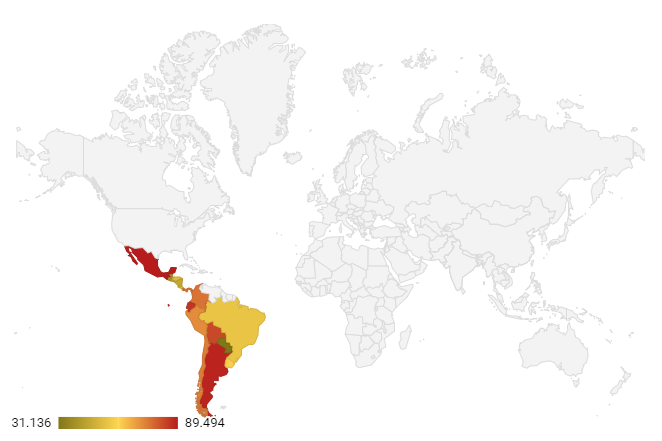
\includegraphics[height=0.5in]{./img/mapav2.png}
  \caption{Geo-mapa}
  \label{fig:mapav2}
\end{subfigure}%
\begin{subfigure}
  \centering
  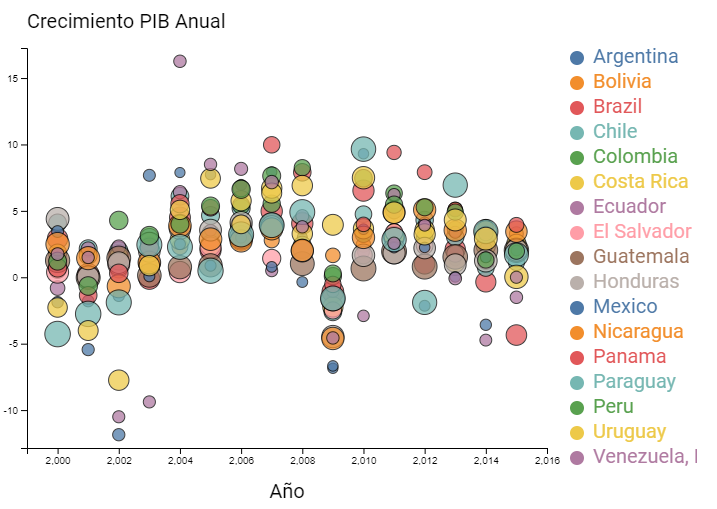
\includegraphics[height=0.5in]{./img/pibv2.png}
  \caption{Gráfico de burbujas}
  \label{fig:pibv2}
\end{subfigure}
\end{figure*}

Los cambios mas significativos se dieron en los gráficos del PIB (figura \ref{fig:pibv2}) y los tipos de energía (figura \ref{fig:tiposv2})

\begin{figure}[H]
\caption{Gráficos representando los indicadores. Versión Final de la visualización.}
% \begin{subfigure}{\textwidth}
%   \centering
%   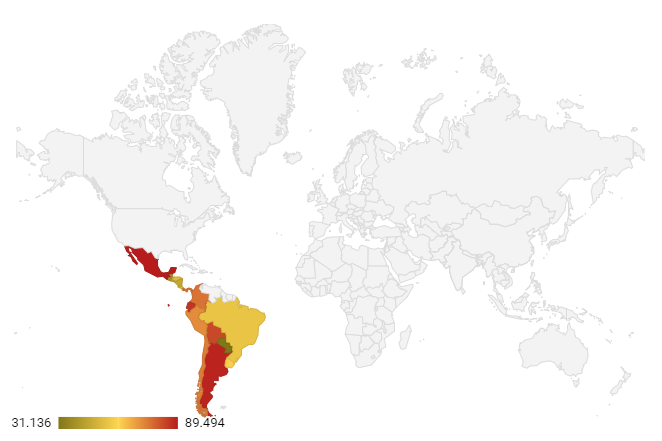
\includegraphics[width=1\linewidth]{./img/mapav2.png}
%   \caption{Geo-mapa con el porcentaje promedio anual del consumo de energías procedentes de hidrocarburos.}
%   \label{fig:mapav2}
% \end{subfigure}%
% \begin{subfigure}{\textwidth}
%   \centering
%   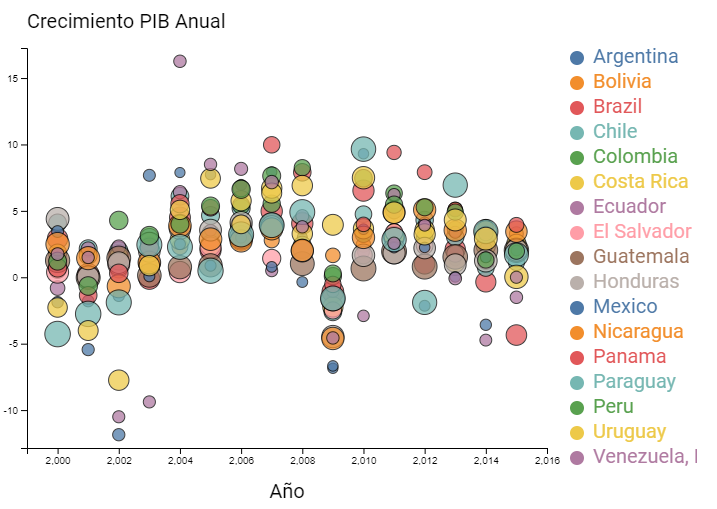
\includegraphics[width=1\linewidth]{./img/pibv2.png}
%   \caption{Gráfico de burbujas relación PIB y producción de energía de fuentes renovables anual por país.}
%   \label{fig:pibv2}
% \end{subfigure}
\begin{subfigure}{\textwidth}
  \centering
  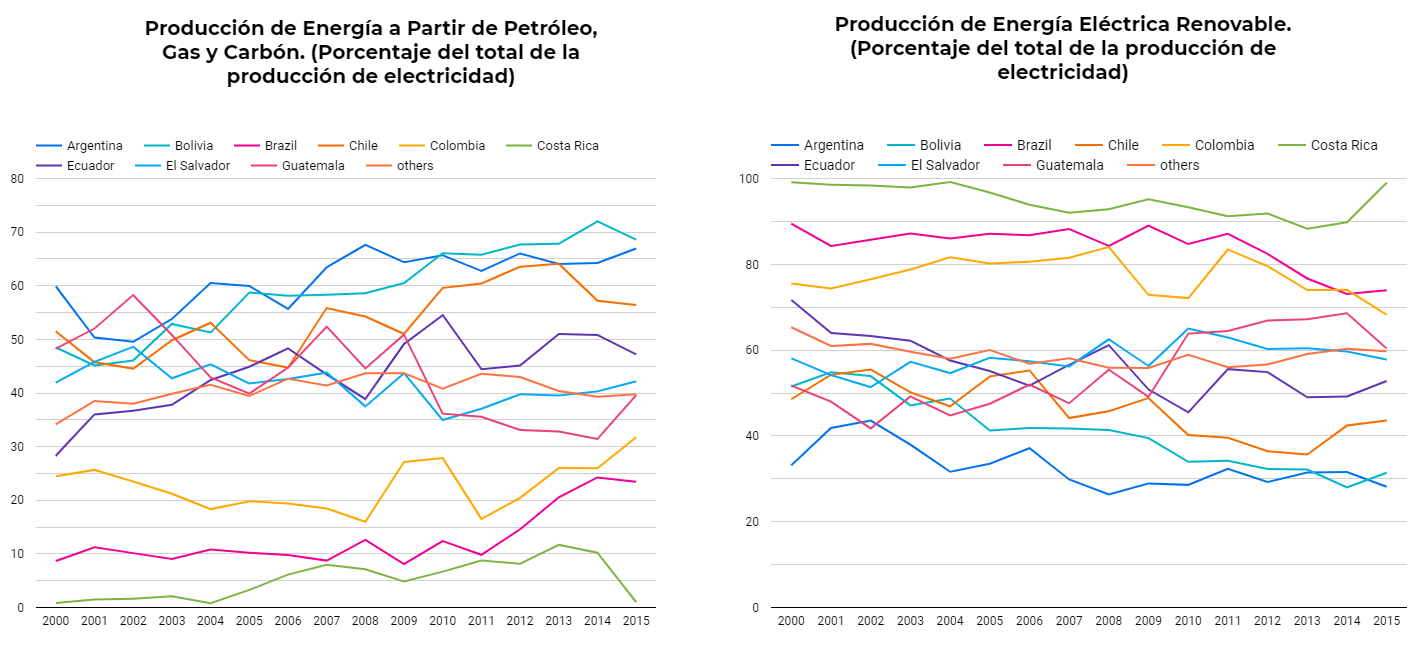
\includegraphics[width=1\linewidth]{./img/prodv2.png}
  \caption{Gráfico de lineas con los porcentajes de producción de energías derivadas del petroleo y renovables respectivamente.}
  \label{fig:prodv2}
\end{subfigure}
\begin{subfigure}{\textwidth}
  \centering
  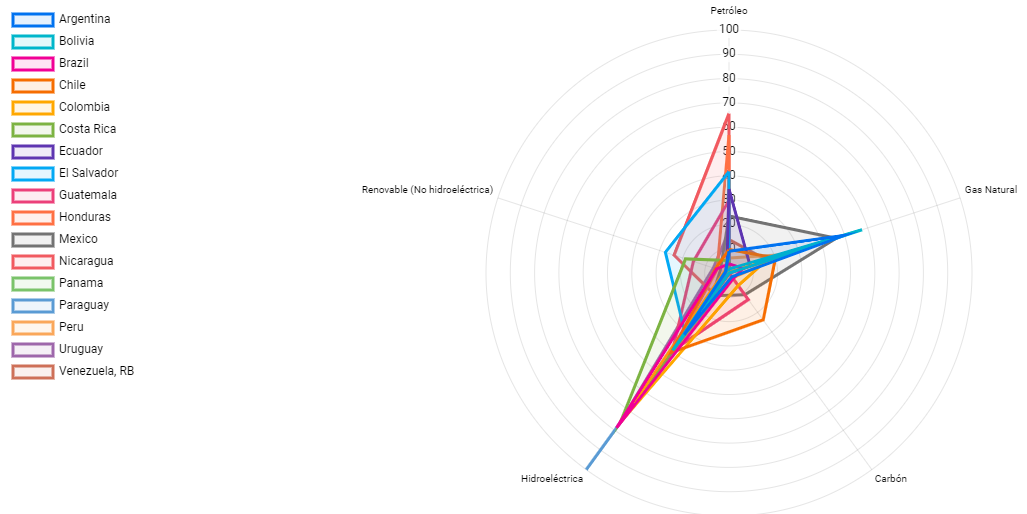
\includegraphics[width=1\linewidth]{./img/spiderv2.png}
  \caption{Gráfico radar representa los porcentajes promedios anuales del tipo de producción de energía por país.}
  \label{fig:tiposv2}
\end{subfigure}
\label{fig:version_2}
\end{figure}



\subsection{Interactuar}

The template is used to format your paper and style the text. All margins, column widths, line spaces, and text fonts are prescribed; please do not alter them. You may note peculiarities. For example, the head margin in this template measures proportionately more than is customary. This measurement and others are deliberate, using specifications that anticipate your paper as one part of the entire proceedings, and not as an independent document. Please do not revise any of the current designations

\section{MATH}

Before you begin to format your paper, first write and save the content as a separate text file. Keep your text and graphic files separate until after the text has been formatted and styled. Do not use hard tabs, and limit use of hard returns to only one return at the end of a paragraph. Do not add any kind of pagination anywhere in the paper. Do not number text heads-the template will do that for you.

Finally, complete content and organizational editing before formatting. Please take note of the following items when proofreading spelling and grammar:

\subsection{Abbreviations and Acronyms} Define abbreviations and acronyms the first time they are used in the text, even after they have been defined in the abstract. Abbreviations such as IEEE, SI, MKS, CGS, sc, dc, and rms do not have to be defined. Do not use abbreviations in the title or heads unless they are unavoidable.

\subsection{Units}

\begin{itemize}

\item Use either SI (MKS) or CGS as primary units. (SI units are encouraged.) English units may be used as secondary units (in parentheses). An exception would be the use of English units as identifiers in trade, such as ``3.5-inch disk drive''.
\item Avoid combining SI and CGS units, such as current in amperes and magnetic field in oersteds. This often leads to confusion because equations do not balance dimensionally. If you must use mixed units, clearly state the units for each quantity that you use in an equation.
\item Do not mix complete spellings and abbreviations of units: ``Wb/m2'' or ``webers per square meter'', not ``webers/m2''.  Spell out units when they appear in text: ``\ldots a few henries'', not ``\ldots a few H''.
\item Use a zero before decimal points: ``0.25'', not ``.25''. Use ``cm$^3$'', not ``cc''. (bullet list)

\end{itemize}


\subsection{Equations}

The equations are an exception to the prescribed specifications of this template. You will need to determine whether or not your equation should be typed using either the Times New Roman or the Symbol font (please no other font). To create multileveled equations, it may be necessary to treat the equation as a graphic and insert it into the text after your paper is styled. Number equations consecutively. Equation numbers, within parentheses, are to position flush right, as in (1), using a right tab stop. To make your equations more compact, you may use the solidus ( / ), the exp function, or appropriate exponents. Italicize Roman symbols for quantities and variables, but not Greek symbols. Use a long dash rather than a hyphen for a minus sign. Punctuate equations with commas or periods when they are part of a sentence, as in
\begin{equation}
\alpha + \beta = \chi
\end{equation}

Note that the equation is centered using a center tab stop. Be sure that the symbols in your equation have been defined before or immediately following the equation. Use ``(1)'', not ``Eq. (1)'' or ``equation (1)'', except at the beginning of a sentence: ``Equation (1) is\ldots''

\subsection{Some Common Mistakes}
\begin{itemize}


\item The word ``data'' is plural, not singular.
\item The subscript for the permeability of vacuum ?0, and other common scientific constants, is zero with subscript formatting, not a lowercase letter ``o''.
\item In American English, commas, semi-/colons, periods, question and exclamation marks are located within quotation marks only when a complete thought or name is cited, such as a title or full quotation. When quotation marks are used, instead of a bold or italic typeface, to highlight a word or phrase, punctuation should appear outside of the quotation marks. A parenthetical phrase or statement at the end of a sentence is punctuated outside of the closing parenthesis (like this). (A parenthetical sentence is punctuated within the parentheses.)
\item A graph within a graph is an ``inset'', not an ``insert''. The word alternatively is preferred to the word ``alternately'' (unless you really mean something that alternates).
\item Do not use the word ``essentially'' to mean ``approximately'' or ``effectively''.
\item In your paper title, if the words ``that uses'' can accurately replace the word ``using'', capitalize the ``u''; if not, keep using lower-cased.
\item Be aware of the different meanings of the homophones ``affect'' and ``effect'', ``complement'' and ``compliment'', ``discreet'' and ``discrete'', ``principal'' and ``principle''.
\item Do not confuse ``imply'' and ``infer''.
\item The prefix ``non'' is not a word; it should be joined to the word it modifies, usually without a hyphen.
\item There is no period after the ``et'' in the Latin abbreviation ``et al.''.
\item The abbreviation ``i.e.'' means ``that is'', and the abbreviation ``e.g.'' means ``for example''.

\end{itemize}


\section{USING THE TEMPLATE}

Use this sample document as your LaTeX source file to create your document. Save this file as {\bf root.tex}. You have to make sure to use the cls file that came with this distribution. If you use a different style file, you cannot expect to get required margins. Note also that when you are creating your out PDF file, the source file is only part of the equation. \emph{Your \TeX\ $\rightarrow$ PDF filter determines the output file size. Even if you make all the specifications to output a letter file in the source - if you filter is set to produce A4, you will only get A4 output.}

It is impossible to account for all possible situation, one would encounter using \TeX. If you are using multiple \TeX\ files you must make sure that the ``MAIN`` source file is called root.tex - this is particularly important if your conference is using PaperPlaza's built in \TeX\ to PDF conversion tool.

\subsection{Headings, etc}

Text heads organize the topics on a relational, hierarchical basis. For example, the paper title is the primary text head because all subsequent material relates and elaborates on this one topic. If there are two or more sub-topics, the next level head (uppercase Roman numerals) should be used and, conversely, if there are not at least two sub-topics, then no subheads should be introduced. Styles named ``Heading 1'', ``Heading 2'', ``Heading 3'', and ``Heading 4'' are prescribed.

\subsection{Figures and Tables}

Positioning Figures and Tables: Place figures and tables at the top and bottom of columns. Avoid placing them in the middle of columns. Large figures and tables may span across both columns. Figure captions should be below the figures; table heads should appear above the tables. Insert figures and tables after they are cited in the text. Use the abbreviation ``Fig. 1'', even at the beginning of a sentence.

\begin{table}[h]
\caption{An Example of a Table}
\label{table_example}
\begin{center}
\begin{tabular}{|c||c|}
\hline
One & Two\\
\hline
Three & Four\\
\hline
\end{tabular}
\end{center}
\end{table}



   

Figure Labels: Use 8 point Times New Roman for Figure labels. Use words rather than symbols or abbreviations when writing Figure axis labels to avoid confusing the reader. As an example, write the quantity ``Magnetization'', or ``Magnetization, M'', not just ``M''. If including units in the label, present them within parentheses. Do not label axes only with units. In the example, write ``Magnetization (A/m)'' or ``Magnetization {A[m(1)]}'', not just ``A/m''. Do not label axes with a ratio of quantities and units. For example, write ``Temperature (K)'', not ``Temperature/K.''

\section{Conclusiones}

A conclusion section is not required. Although a conclusion may review the main points of the paper, do not replicate the abstract as the conclusion. A conclusion might elaborate on the importance of the work or suggest applications and extensions. 

\addtolength{\textheight}{-12cm}   % This command serves to balance the column lengths
                                  % on the last page of the document manually. It shortens
                                  % the textheight of the last page by a suitable amount.
                                  % This command does not take effect until the next page
                                  % so it should come on the page before the last. Make
                                  % sure that you do not shorten the textheight too much.

%%%%%%%%%%%%%%%%%%%%%%%%%%%%%%%%%%%%%%%%%%%%%%%%%%%%%%%%%%%%%%%%%%%%%%%%%%%%%%%%



%%%%%%%%%%%%%%%%%%%%%%%%%%%%%%%%%%%%%%%%%%%%%%%%%%%%%%%%%%%%%%%%%%%%%%%%%%%%%%%%



%%%%%%%%%%%%%%%%%%%%%%%%%%%%%%%%%%%%%%%%%%%%%%%%%%%%%%%%%%%%%%%%%%%%%%%%%%%%%%%%
%\section*{APPENDIX}
%
%Appendixes should appear before the acknowledgment.
%
%\section*{ACKNOWLEDGMENT}
%
%The preferred spelling of the word ``acknowledgment'' in America is without an ``e'' after the ``g''. Avoid the stilted expression, ``One of us (R. B. G.) thanks . . .''  Instead, try ``R. B. G. thanks''. Put sponsor acknowledgments in the unnumbered footnote on the first page.
%


%%%%%%%%%%%%%%%%%%%%%%%%%%%%%%%%%%%%%%%%%%%%%%%%%%%%%%%%%%%%%%%%%%%%%%%%%%%%%%%%

References are important to the reader; therefore, each citation must be complete and correct. If at all possible, references should be commonly available publications.

\bibliography{main}{}
\bibliographystyle{acm}




\end{document}
